\documentclass[tikz,convert={outfile=\jobname.svg}]{standalone}
%\usetikzlibrary{...}% tikz package already loaded by 'tikz' option

\usetikzlibrary{3d}          % for 'canvas is...' options
\usetikzlibrary{perspective} % for '3d view' option
\tikzset
{
    linea/.style={draw=red},
    lineb/.style={draw=blue},
}

\renewcommand{\a}{3.2}
\renewcommand{\b}{1.2}

\newcommand{\simplecube}[8]% origin, dimension x, dimension y, dimension z, style x, style y, style z
{
    \begin{scope}[shift={#1}]
        \fill[gray!40,canvas is yz plane at x=#2, opacity=#8] (0,0) rectangle (#3,#4);
        \fill[gray!10,canvas is xz plane at y=#3, opacity=#8] (0,0) rectangle (#2,#4);
        \fill[white  ,canvas is xy plane at z=#4, opacity=#8] (0,0) rectangle (#2,#3);
        \foreach\i/\j in {0/1, 1/1, 1/0}
            {
            \draw[line#5] (0,#3*\i,#4*\j) --++ (#2,0,0);
            \draw[line#6] (#2*\i,0,#4*\j) --++ (0,#3,0);
            \draw[line#7] (#2*\i,#3*\j,0) --++ (0,0,#4);
        }
    \end{scope}
}

\newcommand{\threeSquares}[4]% origin, a, b, separation
{
    \begin{scope}
        \simplecube{(0,     0,      0)}     {1}{1}{1}   {a}{a}{a}   {1}
    \end{scope}
    \begin{scope}
        \simplecube{(0,     0,      0)}     {1}{3}{3}   {a}{a}{a}   {1}
        \simplecube{(1,   0,      0))}    {1}{3}{3}   {a}{a}{a}   {1}
        \simplecube{(2,   0,      0))}    {1}{3}{3}   {a}{a}{a}   {1}
    \end{scope}
    \begin{scope}
        \simplecube{(0,     0,      0)}     {1}{5}{5}   {a}{a}{a}   {1}
        \simplecube{(1,     0,      0)}     {1}{5}{5}   {a}{a}{a}   {1}
        \simplecube{(2,     0,      0)}     {1}{5}{5}   {a}{a}{a}   {1}
        \simplecube{(3,     0,      0)}     {1}{5}{5}   {a}{a}{a}   {1}
        \simplecube{(4,     0,      0)}     {1}{5}{5}   {a}{a}{a}   {1}
    \end{scope}
}
\begin{document}
    \begin{subfigure}
        \centering % b = bottom alignment
        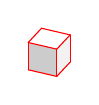
\begin{tikzpicture}[3d view={115}{30},line cap=round,line join=round,scale=0.4]
            \begin{scope}
                \simplecube{(0,     0,      0)}     {1}{1}{1}   {a}{a}{a}   {1}
            \end{scope}
        \end{tikzpicture}
        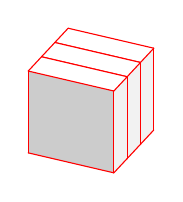
\begin{tikzpicture}[3d view={115}{30},line cap=round,line join=round,scale=0.4]
            \begin{scope}
                \simplecube{(0,     0,      0)}     {1}{3}{3}   {a}{a}{a}   {1}
                \simplecube{(1,   0,      0))}    {1}{3}{3}   {a}{a}{a}   {1}
                \simplecube{(2,   0,      0))}    {1}{3}{3}   {a}{a}{a}   {1}
            \end{scope}
        \end{tikzpicture}
        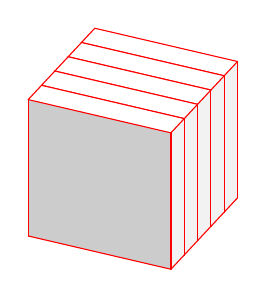
\begin{tikzpicture}[3d view={115}{30},line cap=round,line join=round,scale=0.4]
            \begin{scope}
                \simplecube{(0,     0,      0)}     {1}{5}{5}   {a}{a}{a}   {1}
                \simplecube{(1,     0,      0)}     {1}{5}{5}   {a}{a}{a}   {1}
                \simplecube{(2,     0,      0)}     {1}{5}{5}   {a}{a}{a}   {1}
                \simplecube{(3,     0,      0)}     {1}{5}{5}   {a}{a}{a}   {1}
                \simplecube{(4,     0,      0)}     {1}{5}{5}   {a}{a}{a}   {1}
            \end{scope}
        \end{tikzpicture}
    \end{subfigure}
    \begin{subfigure}
        \centering % b = bottom alignment
        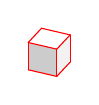
\begin{tikzpicture}[3d view={115}{30},line cap=round,line join=round,scale=0.4]
            \begin{scope}
                \simplecube{(0,     0,      0)}     {1}{1}{1}   {a}{a}{a}   {1}
            \end{scope}
        \end{tikzpicture}
        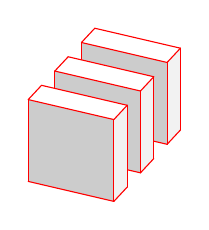
\begin{tikzpicture}[3d view={115}{30},line cap=round,line join=round,scale=0.4]
            \begin{scope}
                \simplecube{(0,     0,      0)}     {1}{3}{3}   {a}{a}{a}   {1}
                \simplecube{(1+1,   0,      0))}    {1}{3}{3}   {a}{a}{a}   {1}
                \simplecube{(2+2*1,   0,      0))}    {1}{3}{3}   {a}{a}{a}   {1}
            \end{scope}
        \end{tikzpicture}
        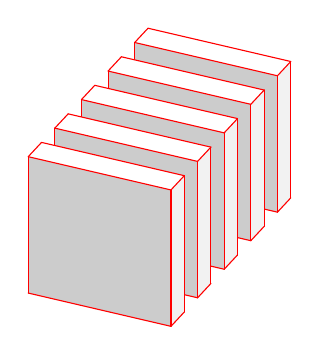
\begin{tikzpicture}[3d view={115}{30},line cap=round,line join=round,scale=0.4]
            \begin{scope}
                \simplecube{(0,     0,      0)}     {1}{5}{5}   {a}{a}{a}   {1}
                \simplecube{(1+1,     0,      0)}     {1}{5}{5}   {a}{a}{a}   {1}
                \simplecube{(2+2*1,    0,      0)}     {1}{5}{5}   {a}{a}{a}   {1}
                \simplecube{(3+3*1,     0,      0)}     {1}{5}{5}   {a}{a}{a}   {1}
                \simplecube{(4+4*1,     0,      0)}     {1}{5}{5}   {a}{a}{a}   {1}
            \end{scope}
        \end{tikzpicture}
    \end{subfigure}
\end{document}